\documentclass[11pt]{article}

\usepackage[margin=1in]{geometry}
\usepackage{amsmath, amssymb, amsthm}
\usepackage{enumitem}
\usepackage{tikz}

\pagestyle{empty}

\begin{document}

\begin{center}
  {\Large\bfseries Weekly Assignment: Variables, Sets,\\[2pt]
   Relations, and Functions (Epp~1.1, 1.2, \& 1.3)}
\end{center}

\bigskip

\noindent
Complete each of the following problems.  Show all work and justify your answers.

\bigskip

%% ─────────────────────────────────────────────
\noindent\textbf{Problem 1} (Epp 1.1 \#2). \;
In each part, fill in the blanks using a variable or variables to
rewrite the given statement.

\medskip\noindent
\emph{Is there an integer that has a remainder of\/ $2$ when it is
divided by\/ $5$ and a remainder of\/ $3$ when it is divided
by\/~$6$?}

\begin{enumerate}[label=\textbf{\alph*.},itemsep=4pt]
  \item Is there an integer $n$ such that $n$~has \rule{2.5cm}{0.4pt}\,?
  \item Does there exist \rule{2.5cm}{0.4pt}\ such that if $n$ is
        divided by~5 the remainder is~2 and if
        \rule{2.5cm}{0.4pt}\,?
\end{enumerate}

\noindent
\emph{Note}: There are integers with this property.
Can you think of one?

\bigskip

%% ─────────────────────────────────────────────
\noindent\textbf{Problem 2} (Epp 1.1 \#4). \;
In each part, fill in the blanks using a variable or variables to
rewrite the given statement.

\medskip\noindent
\emph{Given any real number, there is a real number that is
greater.}

\begin{enumerate}[label=\textbf{\alph*.},itemsep=4pt]
  \item Given any real number~$r$, there is \rule{2.5cm}{0.4pt}\ $s$
        such that $s$~is \rule{2.5cm}{0.4pt}\,.
  \item For any \rule{2.5cm}{0.4pt}\,, \rule{2.5cm}{0.4pt}\ such
        that $s > r$.
\end{enumerate}

\bigskip

%% ─────────────────────────────────────────────
\noindent\textbf{Problem 3} (Epp 1.1 \#7\,b,d). \;
Rewrite the following statements less formally, without using
variables.  Determine, as best as you can, whether each
statement is true or false.

\begin{enumerate}[label=\textbf{\alph*.},start=2,itemsep=4pt]
  \item There is a real number $x$ such that $x^2 < x$.
  \setcounter{enumi}{3}
  \item For all real numbers $a$ and $b$,
        $\;\lvert a + b \rvert \le \lvert a \rvert + \lvert b \rvert$.
\end{enumerate}

\bigskip

%% ─────────────────────────────────────────────
\noindent\textbf{Problem 4} (Epp 1.2 \#2\,b,d). \;
Write in words how to read each of the following out loud.

\begin{enumerate}[label=\textbf{\alph*.},start=2,itemsep=4pt]
  \item $\{x \in \mathbf{R} \mid x \le 0 \text{ or } x \ge 1\}$
  \setcounter{enumi}{3}
  \item $\{n \in \mathbf{Z}^+ \mid n \text{ is a factor of } 6\}$
\end{enumerate}

\bigskip

%% ─────────────────────────────────────────────
\noindent\textbf{Problem 5} (Epp 1.2 \#4). \;
Answer each of the following questions. Give reasons for your
answers.

\begin{enumerate}[label=\textbf{\alph*.},itemsep=4pt]
  \item Is $2 \in \{2\}$?
  \item How many elements are in the set $\{2, 2, 2, 2\}$?
  \item How many elements are in the set $\{0, \{0\}\}$?
  \item Is $\{0\} \in \bigl\{\{0\}, \{1\}\bigr\}$?
  \item Is $0 \in \bigl\{\{0\}, \{1\}\bigr\}$?
\end{enumerate}

\bigskip

%% ─────────────────────────────────────────────
\noindent\textbf{Problem 6} (Epp 1.3 \#2). \;
Let $C = D = \{-3, -2, -1, 1, 2, 3\}$ and define a relation~$S$
from~$C$ to~$D$ as follows: For every $(x,y) \in C \times D$,
\[
  (x, y) \in S \quad\text{means that}\quad
  \frac{1}{x} - \frac{1}{y} \;\text{ is an integer.}
\]

\begin{enumerate}[label=\textbf{\alph*.},itemsep=4pt]
  \item Is $2\;S\;2$?  Is $(-1)\;S\;(-1)$?
        Is $(3, 3) \in S$?  Is $(3, -3) \in S$?
  \item Write $S$ as a set of ordered pairs.
  \item Write the domain and co-domain of $S$.
  \item Draw an arrow diagram for $S$.
\end{enumerate}

\bigskip

%% ─────────────────────────────────────────────
\noindent\textbf{Problem 7} (Epp 1.3 \#14). \;
Let $C = \{1, 2, 3, 4\}$ and $D = \{a, b, c, d\}$.  Define a function
$G\colon C \to D$ by the following arrow diagram:

\begin{center}
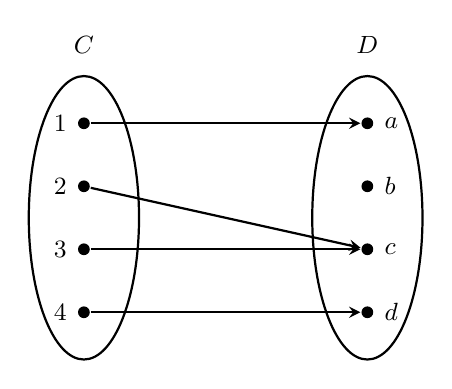
\begin{tikzpicture}[
    dot/.style={circle, fill=black, inner sep=1.5pt},
    every node/.style={font=\small},
    >=stealth,
    thick
  ]
  % Domain oval
  \draw (0,0) ellipse (0.7 and 1.8);
  \node[above] at (0,1.95) {$C$};
  \node[dot, label=left:$1$] (c1) at (0, 1.2) {};
  \node[dot, label=left:$2$] (c2) at (0, 0.4) {};
  \node[dot, label=left:$3$] (c3) at (0,-0.4) {};
  \node[dot, label=left:$4$] (c4) at (0,-1.2) {};

  % Co-domain oval
  \draw (3.6,0) ellipse (0.7 and 1.8);
  \node[above] at (3.6,1.95) {$D$};
  \node[dot, label=right:$a$] (da) at (3.6, 1.2) {};
  \node[dot, label=right:$b$] (db) at (3.6, 0.4) {};
  \node[dot, label=right:$c$] (dc) at (3.6,-0.4) {};
  \node[dot, label=right:$d$] (dd) at (3.6,-1.2) {};

  % Arrows
  \draw[->] (c1) -- (da);
  \draw[->] (c2) -- (dc);
  \draw[->] (c3) -- (dc);
  \draw[->] (c4) -- (dd);
\end{tikzpicture}
\end{center}

\begin{enumerate}[label=\textbf{\alph*.},itemsep=4pt]
  \item Write the domain and co-domain of $G$.
  \item Find $G(1)$, $G(2)$, $G(3)$, and $G(4)$.
\end{enumerate}

\bigskip

%% ─────────────────────────────────────────────
\noindent\textbf{Problem 8} (Proof). \;
Prove that for any equation of the form $y^A + x^B = C$, where
$A$, $B$, and $C$ are positive integers, whether or not the
relation corresponding to this equation is a function (with~$x$
as input and~$y$ as output, over the reals) depends only upon
whether~$A$ is even or odd.

\medskip\noindent
\emph{Hint}: Consider two cases based on the parity of~$A$.
For each case, think about how many real values of~$y$ satisfy
$y^A = C - x^B$ for a given~$x$.  When does a real number have a
unique real $A$th root, and when might it have zero or two?

\end{document}
